\documentclass{article}
\usepackage[superscript,biblabel]{cite}
\usepackage{graphicx}
\usepackage{float}

\graphicspath{{../../analysis/images/}}
\bibliographystyle{plain}

\title{Epistasis is widespread in the genetic control of transcription in humans}


\begin{document}

\maketitle


\begin{abstract}
A long standing question in evolution and human genetics is the extent to which epistasis, the phenomenon whereby one polymorphism's effect on a trait depends on other polymorphisms present in the genome, contributes to complex traits. Though epistasis has been demonstrated in artificial gene manipulation studies in model organisms, and some examples have been shown in other species, few convincing examples exist for epistasis amongst natural polymorphisms in human traits. Its absence from empirical findings may simply be due to its unimportance in the genetic control of complex traits, but we hypothesised that it has previously been too technically difficult to detect due to statistical power and computational issues. Here we show that, using advanced computation techniques and a gene expression study design where any effects are expected to be large, evidence for multiple instances of epistasis is found. In a cohort of 846 individuals with data on 7339 gene expression levels in whole blood, we found that after stringent correction for multiple testing the expression of 249 genes is controlled by 549 significant pairwise epistatic interactions. We attempted replication in two independent datasets and 421 show evidence of significance in at least one dataset. Several genes are controlled by multi-locus epistatic interactions whereby one \emph{cis}-acting single nucleotide polymorphism (SNP) is modulated by several trans-acting SNPs. For example MBNL1 is controlled by an additive effect at rs13069559 which itself is controlled by \emph{trans}-SNPs on 14 different chromosomes, with nearly identical genotype-phenotype (GP) maps for each \emph{cis}-\emph{trans} interaction. Additionally, 69 of the genetic interactions overlap with known chromosome interactions ($p < 1.0 \times 10^{-4}$). This study presents the first strong evidence for the widespread existence of epistasis emerging from natural genetic variation in humans.
\end{abstract}


\section{Main}

\subsection{Introduction}
The past decade has seen a tremendous amount of activity in mapping genetic polymorphisms that underlie complex traits. Typically, SNPs are treated as contributing linearly, independently, and cumulatively to the mean of a trait and this has been successful in identifying hundreds of causal variants. Yet outside the prism of association studies there is widespread evidence for epistasis, not only at the molecular scale in artificial double gene knockouts in experimental organisms but also at the evolutionary scale in fitness adaptation and speciation. Though its importance is frequently the subject of debate, to date there is little convincing empirical evidence for epistasis playing a substantial role in the architecture of complex traits.

The detection of epistasis is hampered by power issues for several reasons, including increased dependence on linkage disequilibrium (LD) between causal SNPs and observed SNPs, increased model complexity in fitting interaction terms, and more extreme significance thresholds to account for increased multiple testing \cite{Hemani2013}. When genetic effect sizes are small, as is expected in most complex traits of interest, the power to detect epistasis diminishes rapidly. There are two ways to overcome this problem, either use extremely large sample sizes, or use traits that are likely to have large effect sizes. Because our focus was to ascertain the extent to which epistasis exists amongst natural genetic variation we opted for the latter approach and searched for epistasis controlling gene expression levels. Though they number in the thousands, these traits are typically heritable but much less polygenic, thus it is expected that any genetic effects will be relatively large, maximising the chance at detecting epistasis should it exist.


\subsection{Initial search in discovery set}
We searched for pairwise epistasis exhaustively in the BSGS dataset, which comprises 846 individuals who are genotyped at 528,509 autosomal SNPs and who have gene expression levels measured in whole blood samples for 7339 genes. Recent hardware and software advances made it possible to perform the $1.03 \times 10^{15}$ statistical tests to complete this analysis. We used permutation analysis to calculate an experiment-wide significance threshold of $2.91 \times 10^{-16}$ at the 5\% family-wise error rate (FWER). SNP pairs were modelled for full genetic effects, including marginal additive and dominance at both SNPs plus four interaction terms. Though we could have used a less complex model to improve statistical efficiency, we deemed it important to be agnostic about the type of epistasis that might exist, and therefore chose not to over-parameterise the test. Because there are many large marginal effects present in these data it was necessary to perform several filtering steps to exclude SNP pairs that were significant due to marginal effects alone. All SNP pairs with LD $r^2 > 0.1$ were removed, and were required to have at least five data points in all nine genotype classes. If multiple SNP pairs were present on the same chromosomes for a particular expression trait then only the sentinal SNP pair was retained. Finally, a nested test contrasting the full genetic model against the marginal additive and dominance model was performed for each remaining SNP pair (Methods), resulting in 549 significant interactions after Bonferroni correction for multiple testing of the filtered SNPs.


\subsection{Replication}
Though a necessary step to establish the veracity of the signals from the discovery set, it is theoretically difficult to replicate epistasis because the dependence on LD between observed SNPs and causal variants is on average four orders of magnitude higher than it is for independent additive effects. The significant SNP pairs were carried forward for replication in two independent datasets that used the same expression assays for analysing transcription in whole blood, Fehrmann ($n=1240$) and EGCUT ($n=891$). There was substantial evidence for overlap of interaction effects in all three datasets. Of the 480 original pairs that passed filtering in Fehrmann and EGCUT, 421 of the SNP pairs showed replication for the interaction test at the 5\% false discovery rate (FDR) level in at least one dataset, and 148 in both datasets (Supplementary Figure \ref{fig:qqplotfdr}). The congruence of the epistatic networks in discovery and replication datasets is shown in Figure \ref{fig:fireworks}. We also report that 39 of the interactions from the discovery set were significant at the Bonferroni level in at least one replication set (Supplementary Figure \ref{fig:qqplotbonf}), and 18 were significant in both. The GP maps for these interactions are remarkably similar in all three datasets (Figure \ref{fig:gpmaps}). We also attempted replication in the CHDWB dataset, but only 185 of the SNP pairs passed filtering because the sample size was small ($n=139$), and due to insufficient power there was no evidence for replication.


\subsection{Functional annotation}
Of the 549 interactions, 66 were \emph{cis}-\emph{cis} acting (both SNPs were on the same chromosome as the expression gene), 470 were \emph{cis}-\emph{trans} acting, and 13 were \emph{trans}-\emph{trans} acting. In total the 549 interactions comprised 835 unique SNPs, which we analysed for functional enrichment. We observed that there was significant enrichment of \emph{cis}-acting SNPs in transcriptionally active regions for haematopoetic cell lines only, as measured by localisation within H3K4me3 active regions (the three tissues with the strongest enrichment are significant at $p < 1 \times 10^{-4}$, after adjusting for multiple testing, Supplementary Figure \ref{fig:transh3k4me3}), but \emph{trans}-acting SNPs did not show tissue specific enrichment ($p > 0.1$ for all tissues, Supplementary Figure \ref{fig:transh3k4me3}). 

We cross referenced our list of interactions with a map of chromosome interacting regions in K562 blood cell lines. Forty-nine epistatic interactions mapped to within 500kb of a chromosome interaction, and 69 mapped to within 2Mb ($p < 1.0 \times 10^{-4}$ in both cases, Supplementary Figure \ref{fig:chromosomeinteractions}). 

There is strong enrichment for SNPs to be localised in enhancer binding regions (Supplementary Figure \ref{fig:enhancers}). This enrichment is consistent for both \emph{cis} and \emph{trans} SNPs.

- General enrichment for regulatory motif modifications

- Names of specific factors that are enriched.

- Functional annotation shows that proteins are not being changed at the codon level


\subsection{Patterns of epistasis}
Though seldom the focus of association studies, SNPs with known main effects are often tested for additive $\times$ additive genetic interactions, but our analysis shows this is unlikely to be sufficient. The majority of interactions comprised of one SNP that had a previously known association and one that had no previous association (476 out of 549). Only 9 interactions were between SNPs that both had marginal effects and 64 were between SNPs that had no known marginal effects. Additionally, we observed that the largest epistatic variance component for the 529 interactions were proportionately divided amongst additive $\times$ additive, additive $\times$ dominance and dominance $\times$ dominance terms ($p = 0.22$ for divergence from expectation). This is expected as these traditional epistatic variance components are statistical formulations rather than biologically meaningful patterns.

We observed a wide range of significant GP maps (Figure \ref{fig:gpmaps}) but the most common form of epistasis detected involved a \emph{trans}-SNP masking the effect of an additive \emph{cis}-SNP. For example, MBNL1 has a \emph{cis} effect at rs13069559 which in turn is controlled by 14 \emph{trans}-SNPs that exhibit a masking pattern such that when the \emph{trans}-SNP is homozygous for the masking allele the decreasing allele of the \emph{cis}-SNP no longer has an affect. Each of these interactions have evidence for replication in at least one dataset and eight have evidence for replication in both datasets. Though the exact mechanism underlying this interaction requires further research, we observed that nine of the 14 \emph{trans} SNPs are located in intronic regions (significantly enriched, $p = 3.11 \times 10^{-9}$) and MBNL1 is involved in RNA modification and regulation of splicing, suggesting a putative mechanism by which epistatic interactions may regulate transcription.


\subsection{Contribution of epistatic variance}
Though we have discovered many instances of epistasis, quantifying the relative importance of epistasis remains an open question. In this study we are able to identify 249 probes with at least one significant interaction given our experiment-wide threshold. Using the same threshold ($p < 2.91 \times 10^{-16}$) for the same data searching for only additive or dominance effects returns 517 probes out of the 7339 analysed with at least one significant effect, therefore the number of instances of epistasis are substantial. However, although many epistatic effects are observed, in terms of their contribution to complex traits a more important metric is the proportion of the variance that they explain. Ideally one would assess this question from a whole genome level but this is intractable for non-additive variance outside of in humans, but quantifying the ascertained effects detected in this study demonstrates that additive variance is overall a much larger component than epistatic variance. We observe that of the significant interactions the average additive contribution to the total phenotypic variance is 11.3\%, over three times higher than the epistatic contribution of 3.7\% (Figure \ref{fig:variancecomponents}). From an experiment-wide perspective, the proportion of the total phenotypic variance of all 7339 probes explained by additive effects significant at the $p < 2.91 \times 10^{-16}$ threshold is 1.9\%, whereas the epistatic signals detected in this study only explains 0.27\%. It must be stressed that this comparison strongly favours additive variance because the power of a 1 d.f. test exceeds that of an 8 d.f. test, and the non-additive variance at causal variants is expected to be grossly underestimated by observed SNPs in comparison to estimates for additive variance.


\subsection{Discussion}
Most genetic studies focus on the additive effects of polymorphisms, and there is a 




\clearpage
\section{Figure legends}

\begin{figure}[H]
	\caption{\textbf{Replication of epistatic networks in two cohorts} Panel A shows the overall network of genetic interactions (edges) for each probe (red nodes) and their controlling SNPs (black nodes) from the discovery set. Panel B shows those interactions that were present at the 5\% FDR level in at least one replication dataset, and panel C shows which interactions were significant in both replication datasets.}
	\label{fig:fireworks}
\end{figure}

\begin{figure}[H]
	\caption{\textbf{Replication of genotype-phenotype maps in two cohorts} The GP maps for each epistatic interaction that is significant at the Bonferroni level in both replication datasets are shown. Each tile represents the expression level for that two-locus genotype class. Phenotypes for each interaction within each cohort are scaled to be between 0 and 1. Phenotypes are for gene transcript levels, where the gene's name is labelled in the panel columns. Panel rows are labelled for the dataset. There is a general trend of the GP maps replicating across all three datasets.}
	\label{fig:gpmaps}
\end{figure}

\begin{figure}[H]
	\caption{\textbf{Comparison of genetic variances} Panel A shows the proportion of phenotypic variation that is captured by additive, dominant and interaction components for all 529 significant interactions, ordered by total phenotypic variance explained by the SNP pair. Panel B shows the proportion of the genetic variance that is attributable to the three variance components, ordered by the proportion that is additive.}
	\label{fig:variancecomponents}
\end{figure}


\clearpage
\section{Figures}
\setcounter{figure}{0}

\begin{figure}[H]
	\centering
	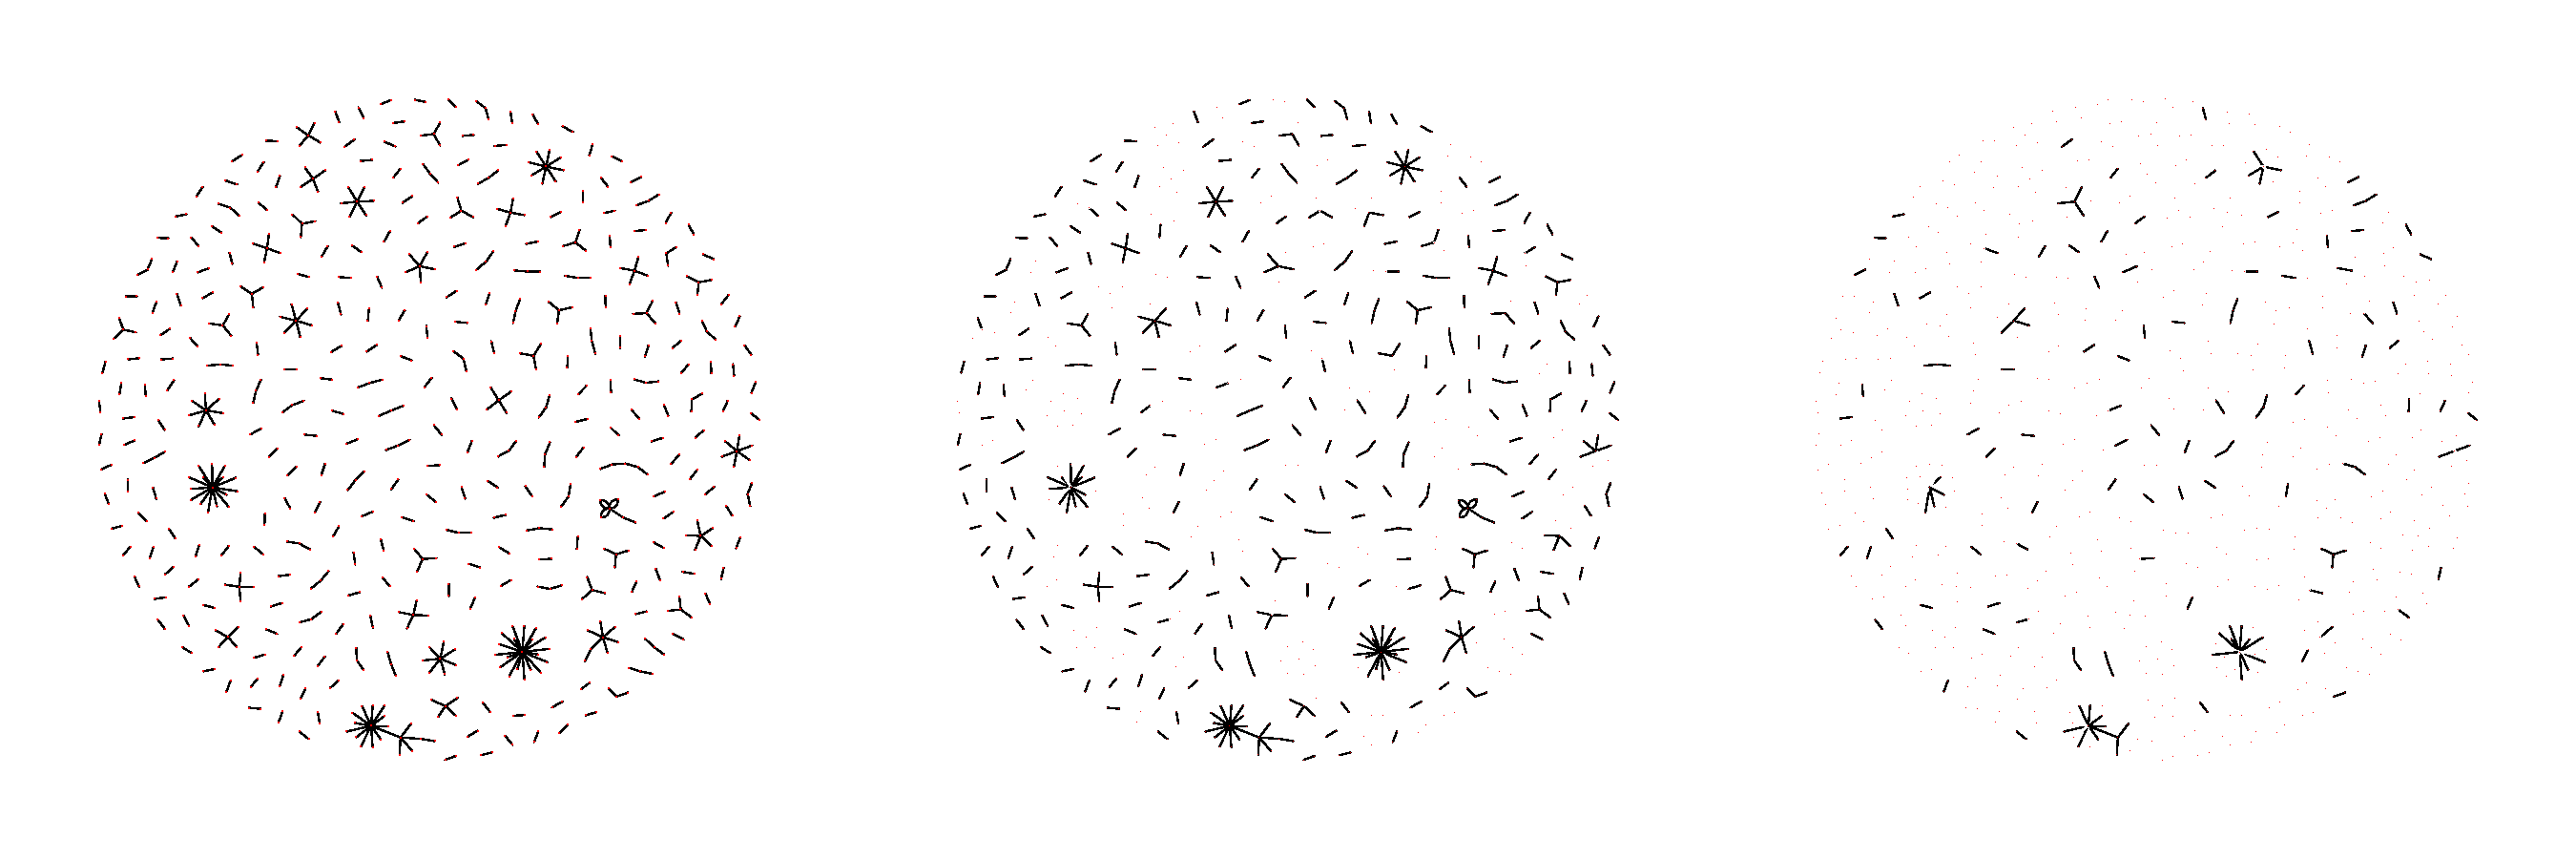
\includegraphics[width=5in]{hairballs_all_reps.pdf}
	\caption{}
\end{figure}
\clearpage

\begin{figure}
	\centering
	\includegraphics[width=5in]{gpbonfrep.pdf}
	\caption{}
\end{figure}
\clearpage

\begin{figure}
	\centering
	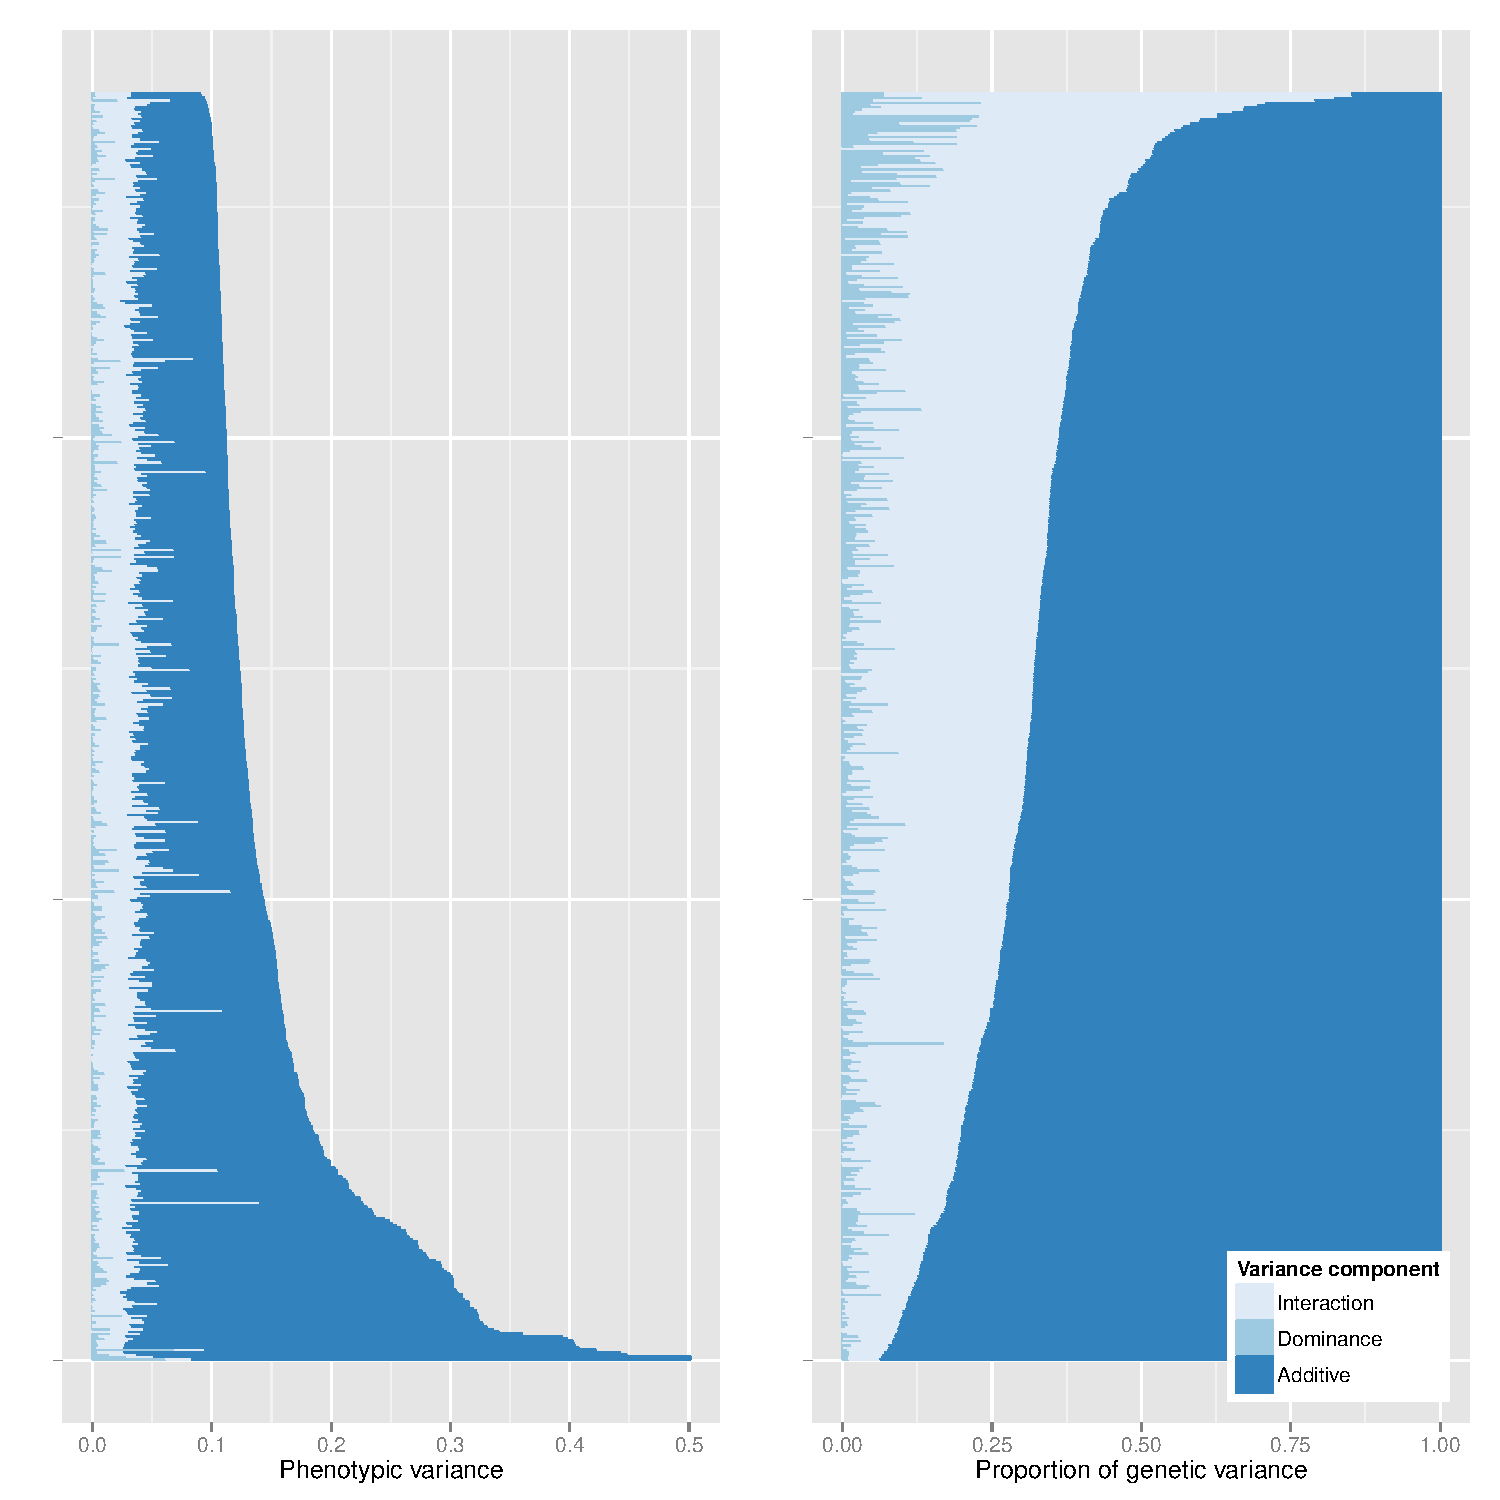
\includegraphics[width=5in]{variance_components.pdf}
	\caption{}
\end{figure}
\clearpage

\section{Full Methods}

\subsection{Discovery data}

The Brisbane Systems Genetics Study (BSGS) comprises 846 individuals of European descent from 274 independent families \cite{pmid22563384}. DNA samples from each individual were genotyped on the Illumina 610-Quad Beadchip by the Scientific Services Division at deCODE Genetics Iceland. Full details of genotyping procedures are given in Medland et al. \cite{Medland2009} Standard QC filters were applied and the remaining 528,509 autosomal SNPs were carried forward for further analysis. 

Gene expression profiles were generated from whole blood collected with PAXgene TM tubes (QIAGEN, Valencia, CA) using Illumina HT12-v4.0 bead arrays. The Illumina HT-12 v4.0 chip contains 47,323 probes, although some probes are not assigned to RefSeq genes. We removed any probes that did not match the following criteria: contained a SNP within the probe sequence with MAF > 0.05 within 1000 genomes data; did not map to a listed ref-seq gene; were not significantly expressed (based on a detection $p$-value $< 0.05$) in at least 90\% of samples. After this stringent QC 7339 probes remained for 2D-eQTL mapping.


\subsection{Normalisation}

Gene expression profiles were normalised and adjusted for batch and polygenic effects. Profiles were first adjusted for raw background expression in each sample. Expression levels were then adjusted using quantile and log2 transformation to standardise distributions between samples. Batch and polygenic effects were adjusted using the linear model

\begin{equation}
y = \mu + \beta_{1}c + \beta_{2}p + \beta_{3}s + \beta_{4}a + g + e
\label{eq:lm}
\end{equation}
where $\mu$ is the population mean expression levels, $c$, $p$, $s$ and $a$ are vectors of chip, chip position, sex and generation respectively, fitted as fixed effects; and $g$ is a random additive polygenic effect with a variance covariance matrix 
\begin{equation}
G_{ijk} = \left \{ 
\begin{array}{ll}
\sigma _a ^2 + \sigma _e ^2&        j = k \\ 
2\phi _{ijk} \sigma _a ^2& 			j \neq k \\
\end{array} \right.
\end{equation}
The parameters $\sigma_a^2$ and $\sigma_e^2$ are variance components for additive background genetic and environmental effects respectively. Here, we are using family based pedigree information rather than SNP based IDB to account for relationships between individuals and so $\phi _{ijk}$ is the kinship coefficient between individuals $j$ and $k$. The residual, $e$, from equation \ref{eq:lm} is assumed to follow a multivariate normal distribution with a mean of zero. Residuals were normalised by rank transformation and used as the adjusted phenotype for the pairwise epistasis scan. 


\subsection{Exhaustive 2D-eQTL analysis}

We used epiGPU software to perform an exhaustive scan for pairwise interactions, such that each SNP is tested against all other SNPs for statistical association with the expression values for each of the 7339 probes. For each SNP pair there are 9 possible genotype classes. We treat each genotype class as a fixed effect and fit an 8 d.f. $F$-test to test the following hypotheses:

\begin{equation}
H _0 : \sum _{i=1} ^3 \sum _{j=1} ^3 (\bar x _{ij} - \mu) ^2 = 0; 
\end{equation}

\begin{equation}
H _1 : \sum _{i=1} ^3 \sum _{j=1} ^3 (\bar x _{ij} - \mu) ^2 > 0; 
\label{eq:8df}
\end{equation}

where $\mu$ is the mean expression level and $x _{ij}$ is the pairwise genotype class mean for genotype $i$ at SNP 1 and genotype $j$ at SNP 2. This type of test does not parameterize for specific types of epistasis, rather it tests for the joint genetic effects at two loci. This has been demonstrated to be statistically more efficient when searching for a wide range of epistatic patterns, although will include any marginal effects of SNPs.
 
The complete exhaustive scan for 7339 probes comprises $1.03 \times 10^{15}$ $F$-tests. We used permutation analysis to estimate an appropriate significance threshold for the study. To do this we performed a further 1600 exhaustive 2D scans on permuted phenotypes to generate a null distribution of the extreme $p$-values expected to be obtained from this number of multiple tests given the correlation structure between the SNPs. We took the most extreme $p$-value from each of the 1600 scans and set the 5\% FWER to be the 95\% most extreme of these $p$-values, $T_{*} = 2.13 \times 10^{-12}$. The effective number of tests in one 2D scan being performed is therefore $N_{*} = 0.05 / T_{*} \approx 2.33 \times 10^{10}$. To correct for the testing of multiple traits we established an experiment wide threshold of $T = 0.05 / (N_{*} \times 7339) = 2.91 \times 10^{-16}$. This is likely to be conservative as it assumes independence between probes.

Following filtering on this threshold only SNP pairs with at least 5 data points in all 9 genotype classes were kept. We then calculated the LD between interacting SNPs and removed any pairs with $r^2 > 0.1$. If multiple SNP pairs were present on the same chromosomes for a particular expression trait then only the sentinal SNP pair was retained, \emph{i.e.} if a probe had multiple SNP pairs that were on chromosomes one and two then only the SNP pair with the most significant $p$-value was retained. At this stage 6404 filtered SNP pairs remained. We then performed a second filtering screen that was identical to the first but an additional step was included where any SNPs that had previously been shown to have a significant additive or dominant effect ($p < 1.29 \times 10^{-11}$) was removed, creating a second set of 4751 filtered SNP pairs. To ensure that interacting SNPs were driven by epistasis and not marginal effects we performed a nested ANOVA on each filtered pair to test if the interaction terms were significant. We did this by contrasting the full genetic model (8 d.f.) against the reduced marginal effects model which included the additive and dominance terms at both SNPs (4 d.f.). Thus, a 4 d.f. $F$-test was performed on the residual genetic variation, representing the contribution of epistatic variance. Significance of epistasis was determined using a Bonferroni threshold of $0.05 / (6404+4751) = 4.48 \times 10^{-6}$. This resulted in 432 and 117 SNP pairs with significant interaction terms from filters 1 and 2, respectively.


\subsection{Replication}
We have attempted replication of the 529 significant interactions from the discovery set using three independent cohorts; Fehrmann, EGCUT, and CHDWB. Details of the cohorts are as follows.  

\paragraph{Fehrmann: $n=1240$}
The Fehrmann dataset consists of whole peripheral blood samples of 1240 unrelated individuals from the United Kingdom and the Netherlands. Some of these individuals are patients, while others are healthy controls. Individuals were genotyped using the Illumina 610 Quad platform. RNA levels were quantified using the HT12v3 platform.

\paragraph{EGCUT: $n=891$}
The Estonian Genome Center of the University of Tartu (EGCUT) study consists of whole blood samples of 891 unrelated individuals from Estonia. They were genotyped using the Illumina 610 Quad platform. RNA levels were quantified using the HT12v3 platform.

\paragraph{CDHWB: $n=139$}
The Center for Health Discovery and Well Being (CDHWB) Study is a population based cohort consisting of 139 individuals of European descent collected in Atlanta USA. Gene expression profiles were generated with Illumina HT-12 V3.0 arrays from whole blood collected from Tempus tubes that preserve RNA. Whole genome genotypes were measured using Illumina OmniQuad arrays.


\clearpage
\section{References}
\bibliography{refs}


\clearpage
\section{Supplementary Figures}
\setcounter{figure}{0}
\makeatletter 
\renewcommand{\thefigure}{S\@arabic\c@figure} 
\makeatletter 

\begin{figure}[H]
	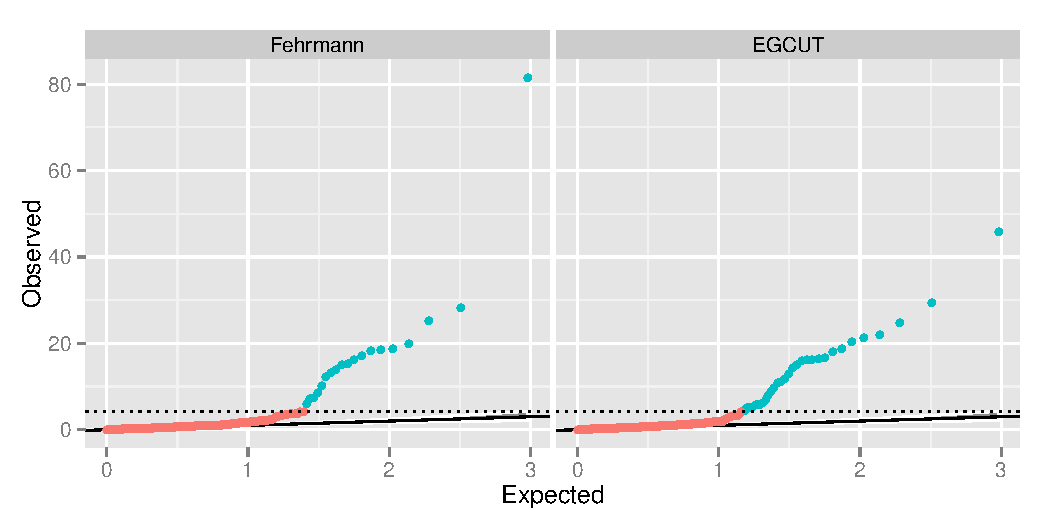
\includegraphics[width=5in]{qqbonf}
	\caption{\textbf{Q-Q plots of interaction $p$-values in two independent datasets} The interaction $p$-values for the 480 SNP pairs that passed filtering in the two replication datasets. Green points represent $p$-values that surpass Bonferroni correction}
	\label{fig:qqplotbonf}
\end{figure}
\clearpage

\begin{figure}
	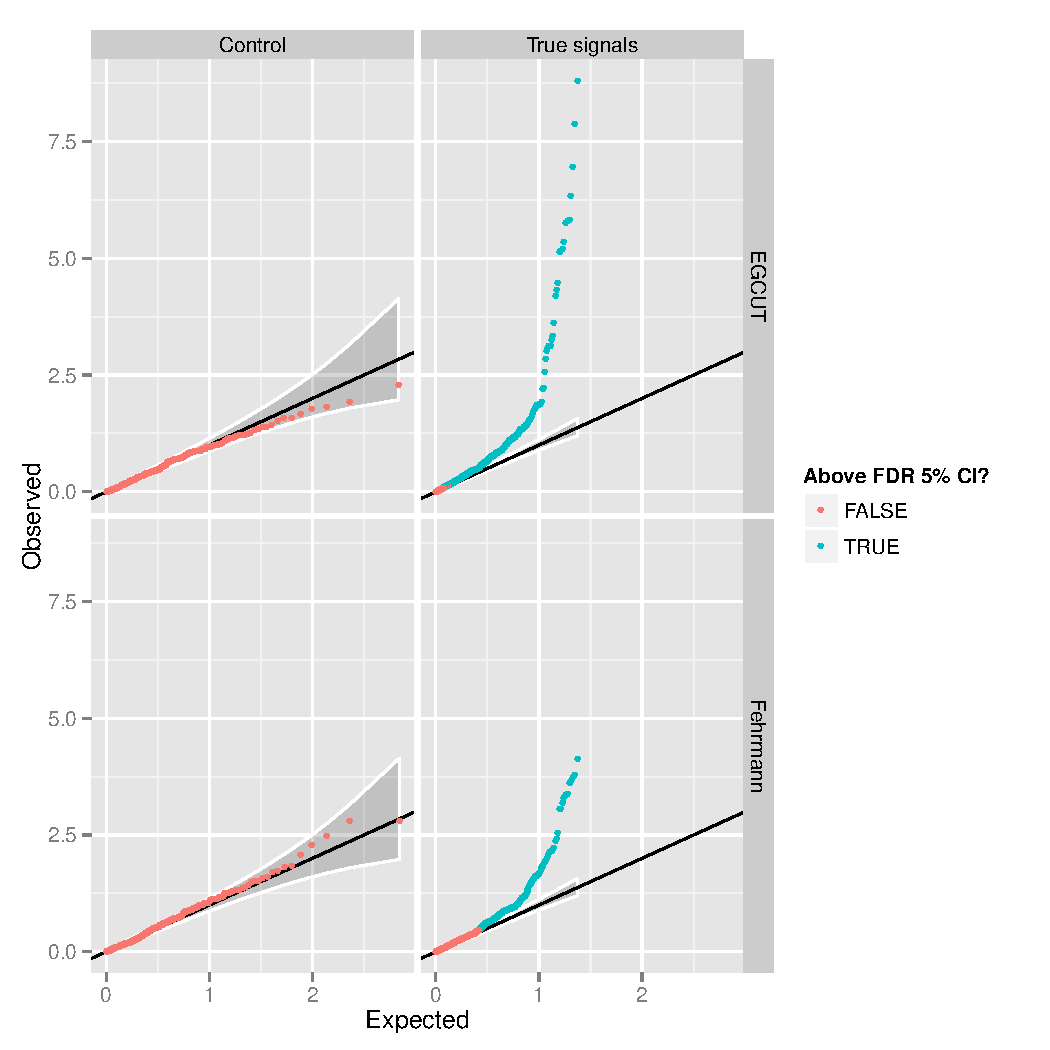
\includegraphics[width=5in]{qqfdr}
	\caption{\textbf{Q-Q plots of replicated interaction $p$-values excluding the 20 most extreme $p$-values} The left panel (Null) shows the replication $p$-values from 529 randomly drawn SNP pairs in the Fehrmann (top row) and EGCUT (bottom row) datasets. The right panel (Observed) shows the interaction $p$-values from the 460 least significant pairs that pass filtering in the two replication datasets (\emph{i.e.} excluding the 20 most extreme $p$-values for clarity). Dark blue points represent $p$-values that surpass the 5\% FDR level.}
\label{fig:qqplotfdr}
\end{figure}
\clearpage

\begin{figure}
	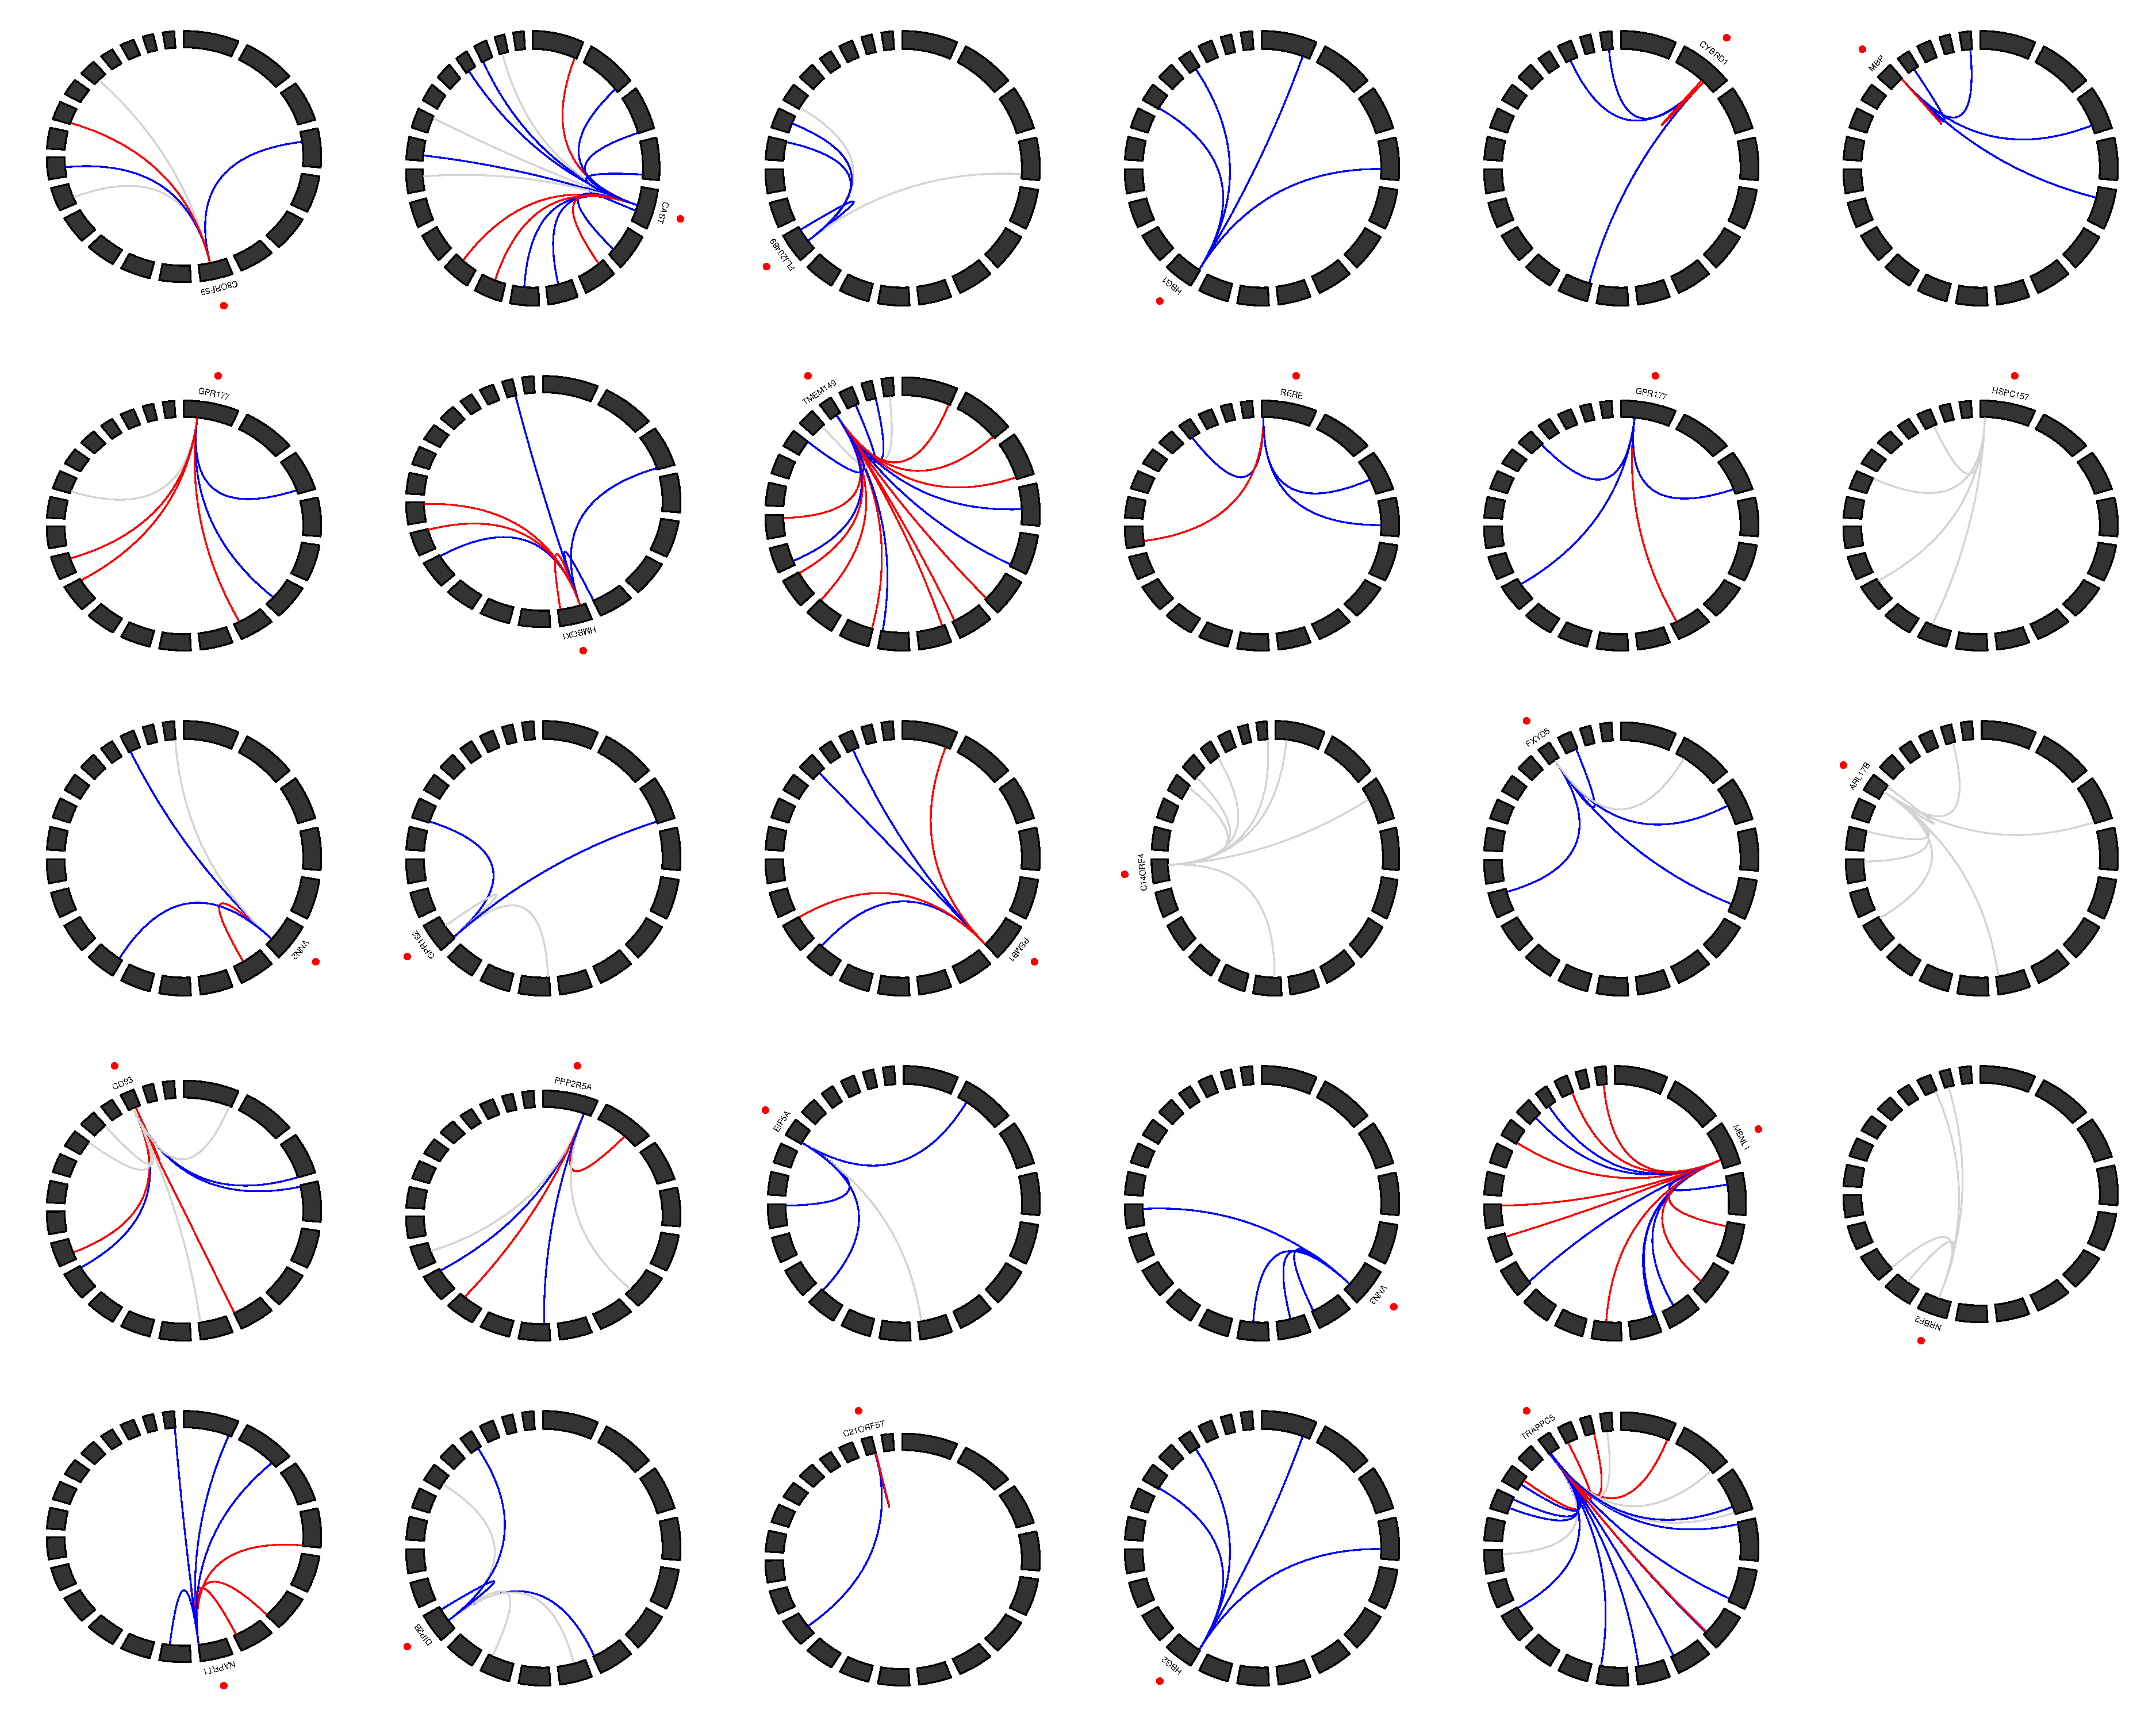
\includegraphics[width=5in]{circles_replication2}
	\caption{\textbf{Gene expression traits with four or more genetic interactions} Circle plots represent the genomic positions for SNPs (linking lines) and expression probes (red points). Chromosomes are represented by black blocks and ordered from 1 to 22 clockwise, starting from the top. Grey lines represent no evidence for replication, blue lines denote replication in at least one dataset, and red lines denote replication in two datasets. Most interactions are characterised as being \emph{cis}-\emph{trans} to the expression probe.}
	\label{fig:circleplots}
\end{figure}
\clearpage

\begin{figure}
	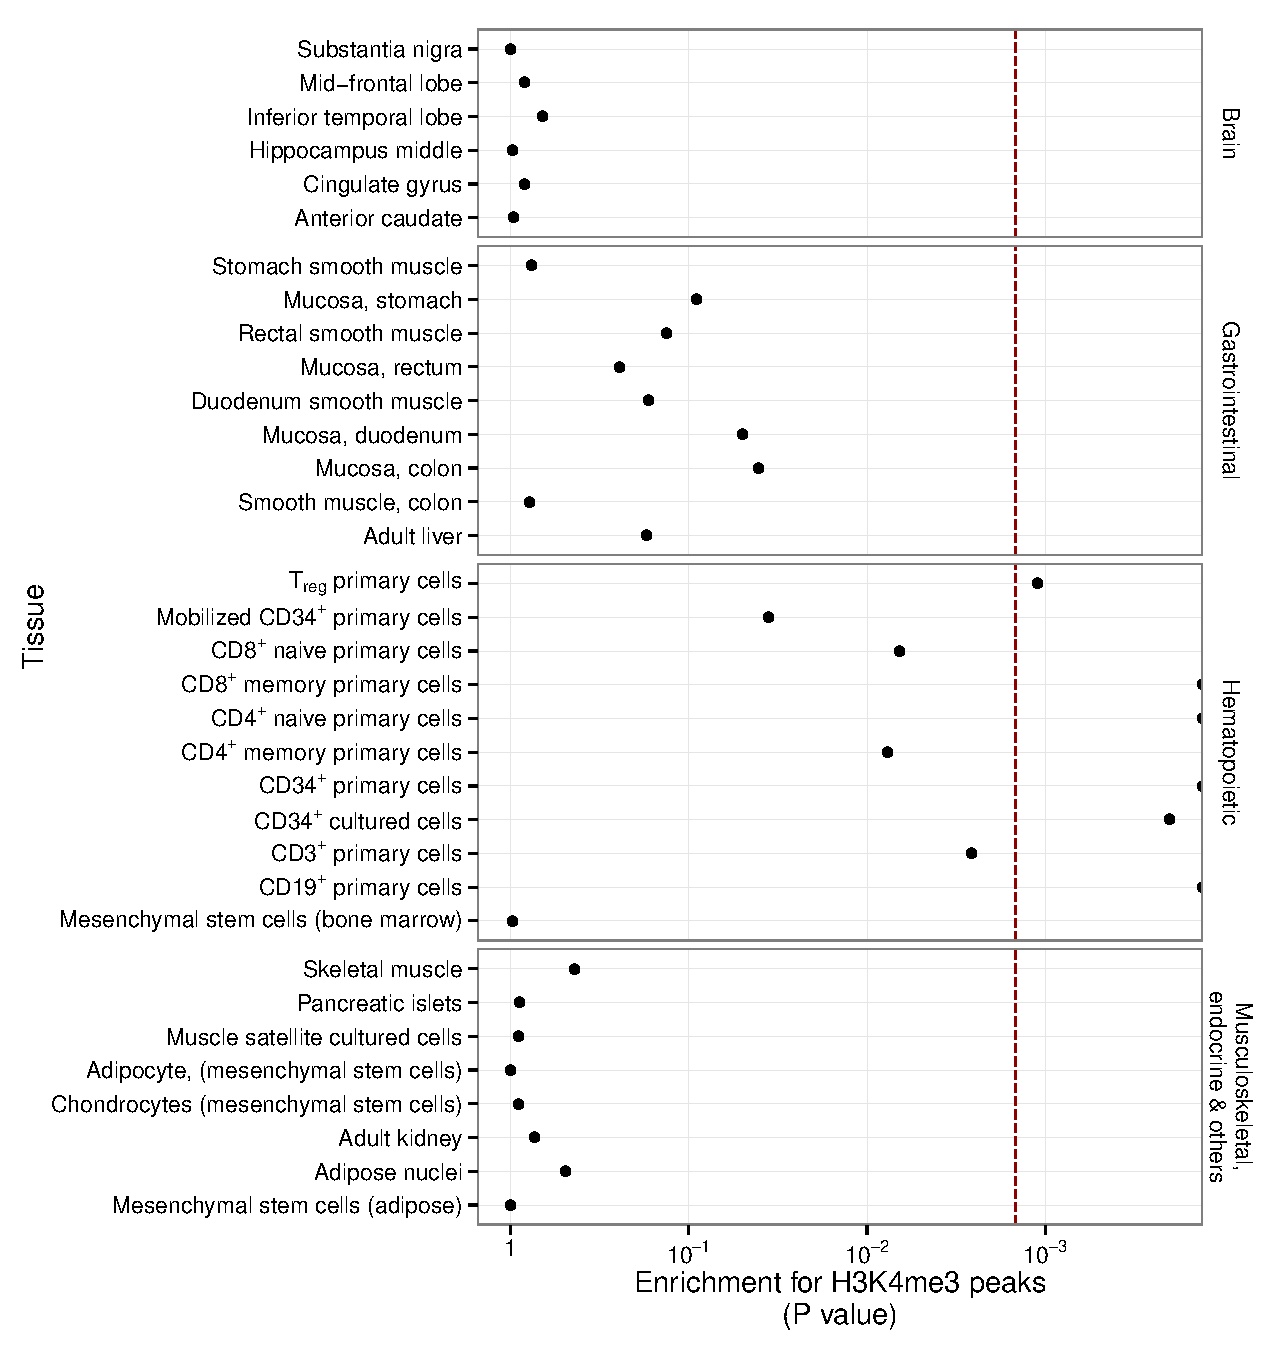
\includegraphics[width=5in]{cis_h3k4me3}
	\caption{\textbf{Tissue specific enrichment of SNPs in transcriptionally active regions} The locations of transcriptional activity can be predicted by chromatin marks, assayed by H3K4me3. Here we show that there is }
	\label{fig:cish3k4me3}
\end{figure}

\begin{figure}
	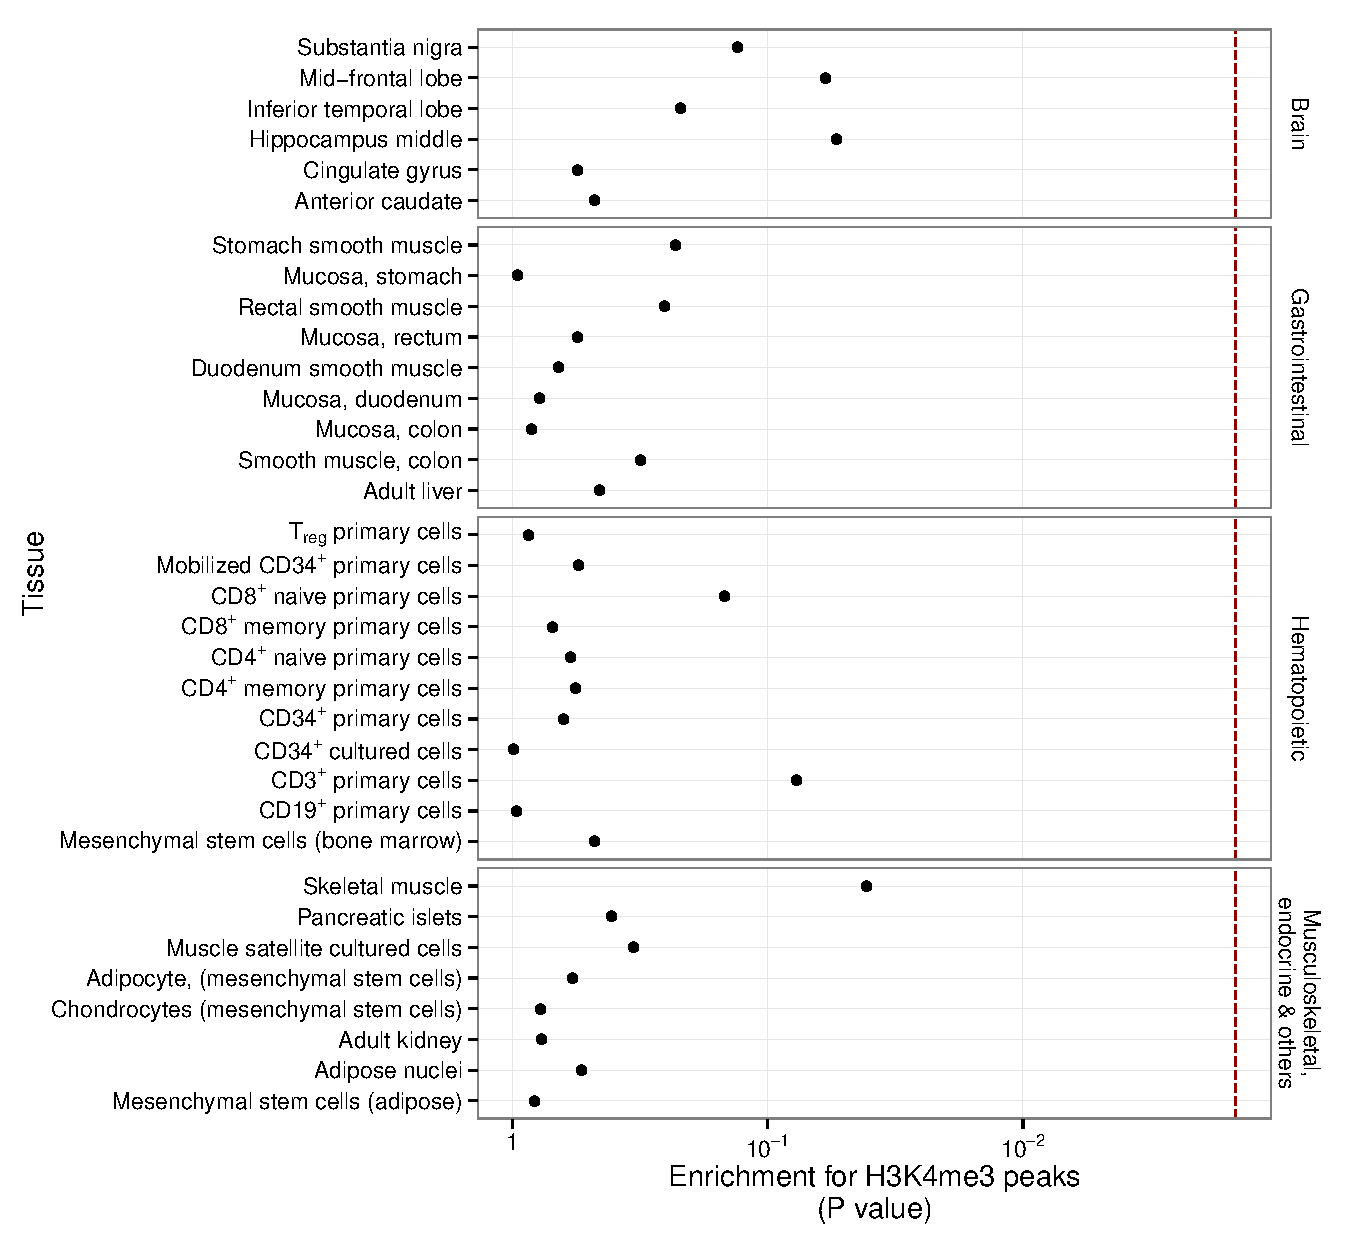
\includegraphics[width=5in]{trans_h3k4me3}
	\caption{\textbf{Tissue specific enrichment of SNPs in transcriptionally active regions} The locations of transcriptional activity can be predicted by chromatin marks, assayed by H3K4me3. Here we show that there is }
	\label{fig:transh3k4me3}
\end{figure}
\clearpage

\begin{figure}
	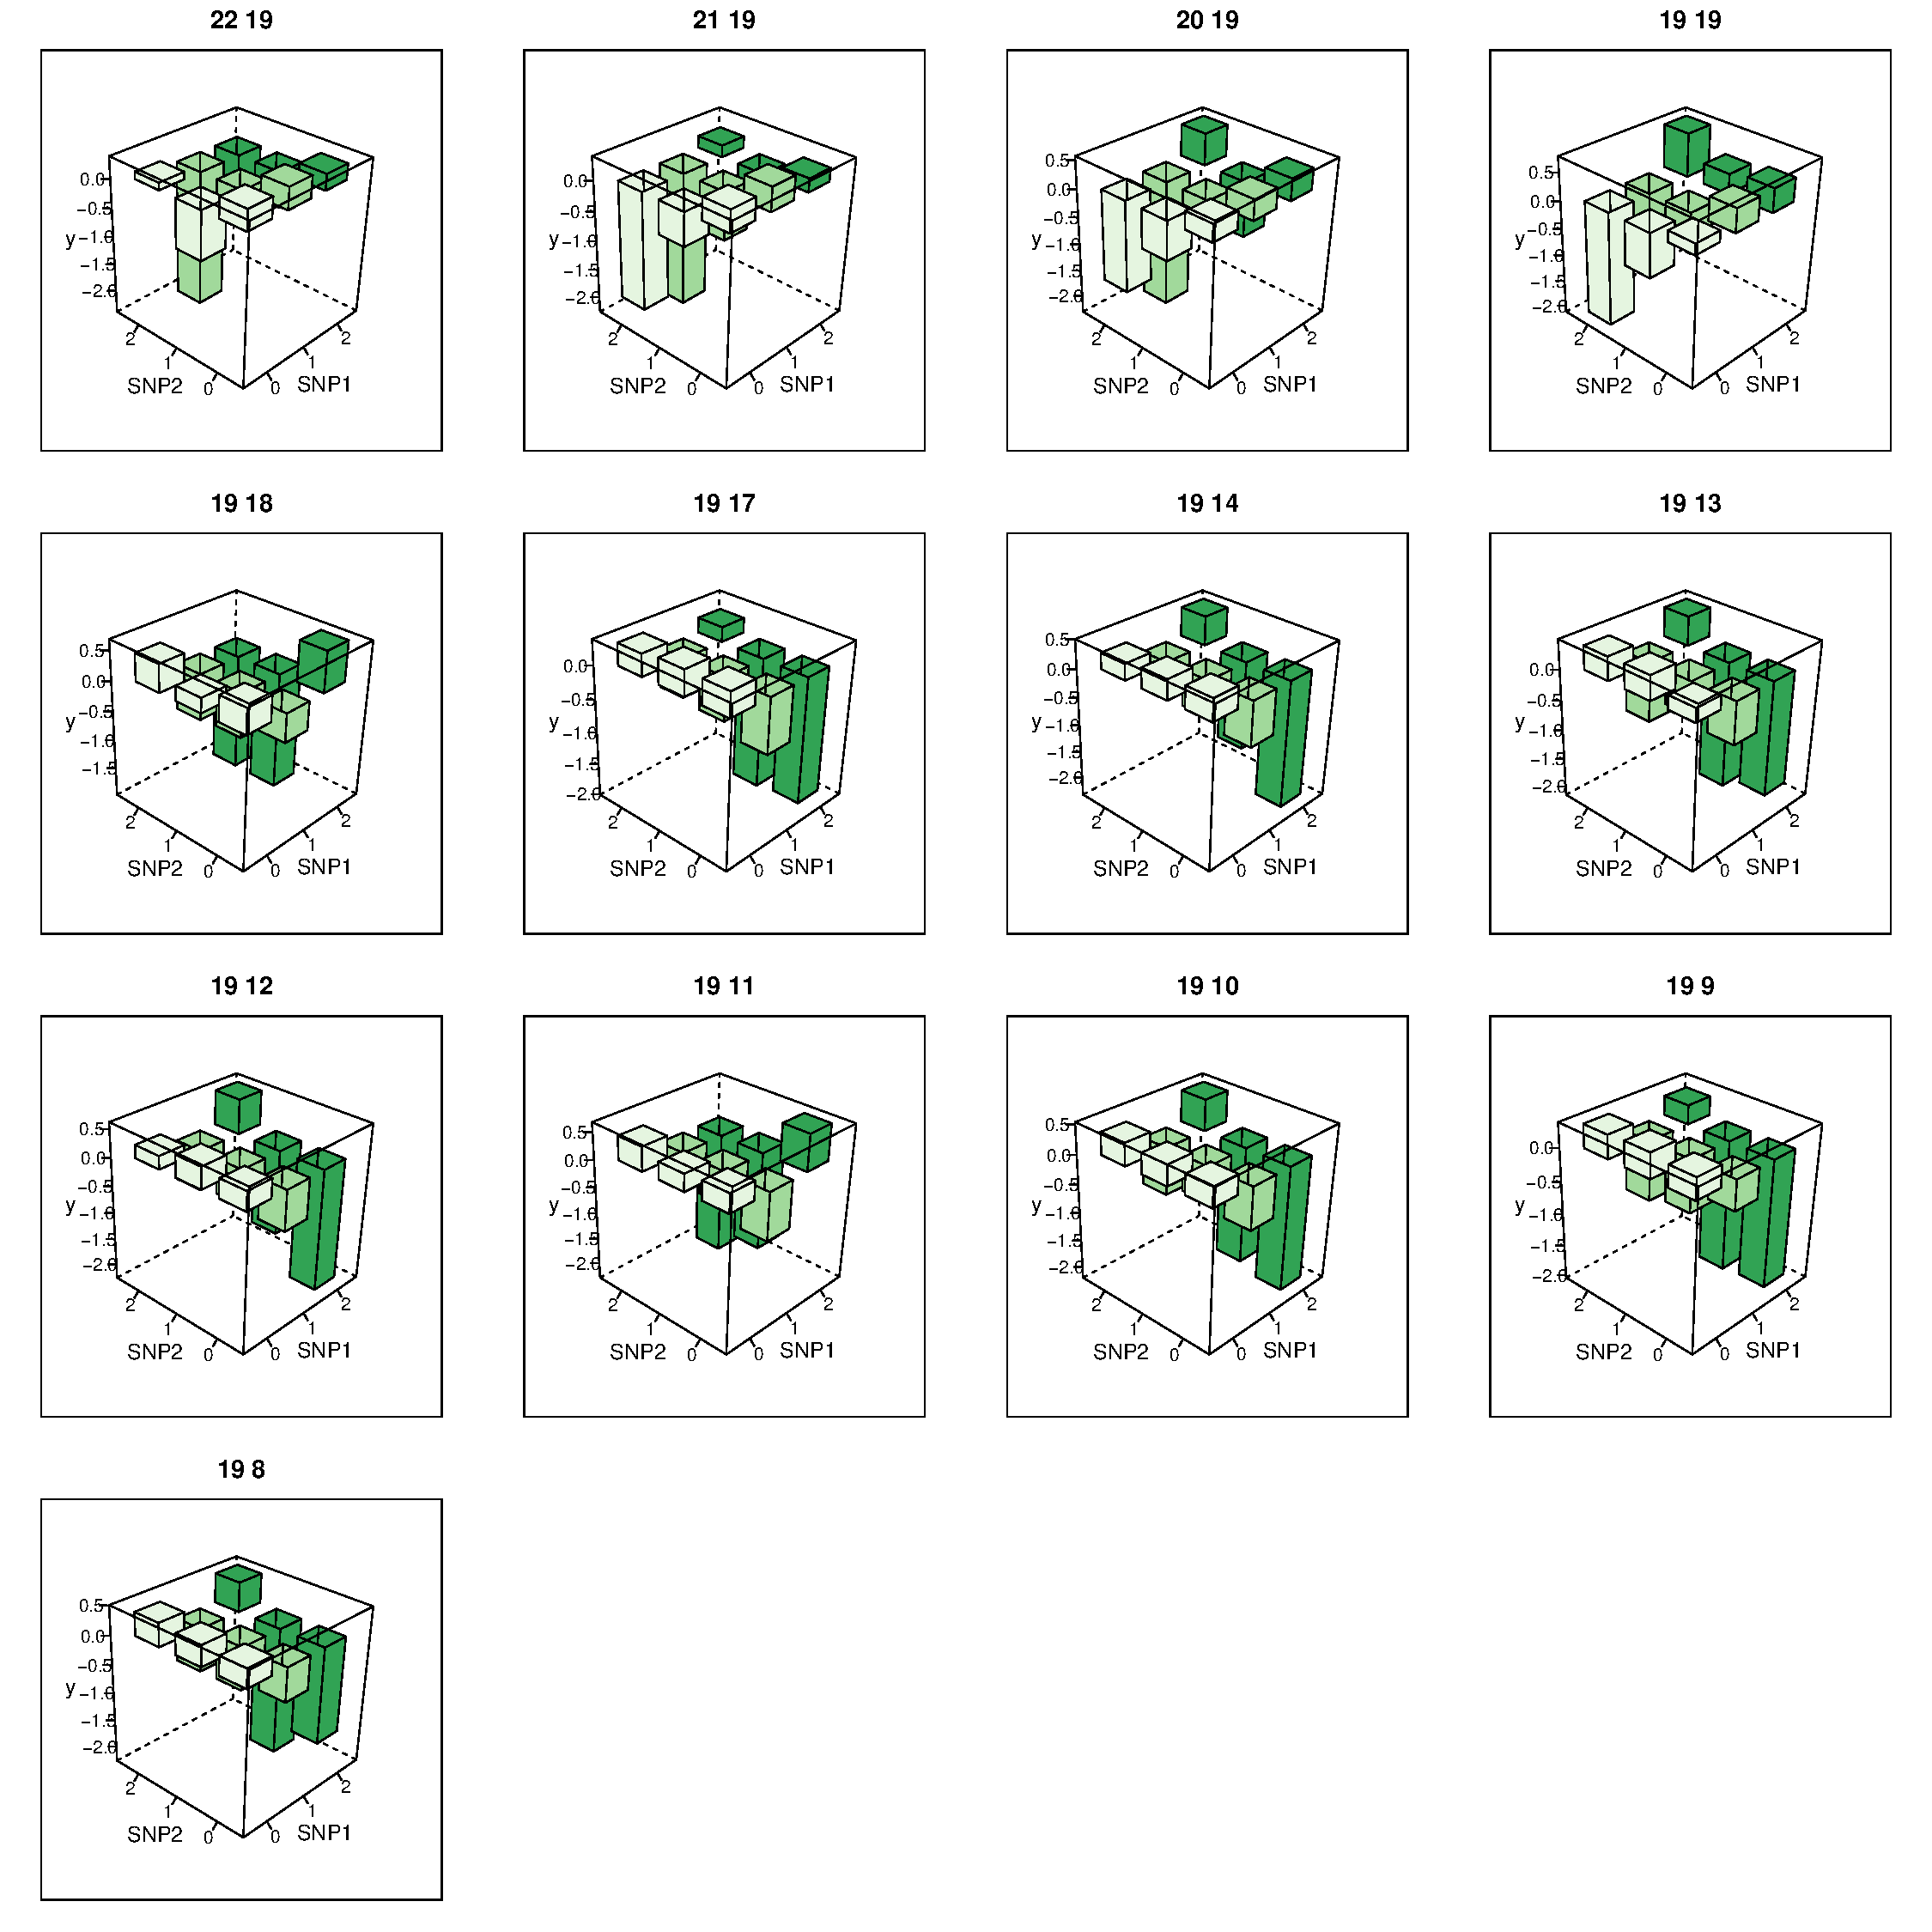
\includegraphics[width=5in]{MBNL1}
	\caption{\textbf{Genotype-phenotype maps for 14 interactions controlling MBNL1} Each bar represents the mean phenotypic value for individuals in that genotype class. The rs13069559 SNP typically has a \emph{cis}-additive decreasing effect on the expression of MBNL1, but in many of these interactions the \emph{cis} effect is masked when the \emph{trans} SNP is homozygous.}
	\label{fig:mbnl13d}
\end{figure}
\clearpage

\begin{figure}
	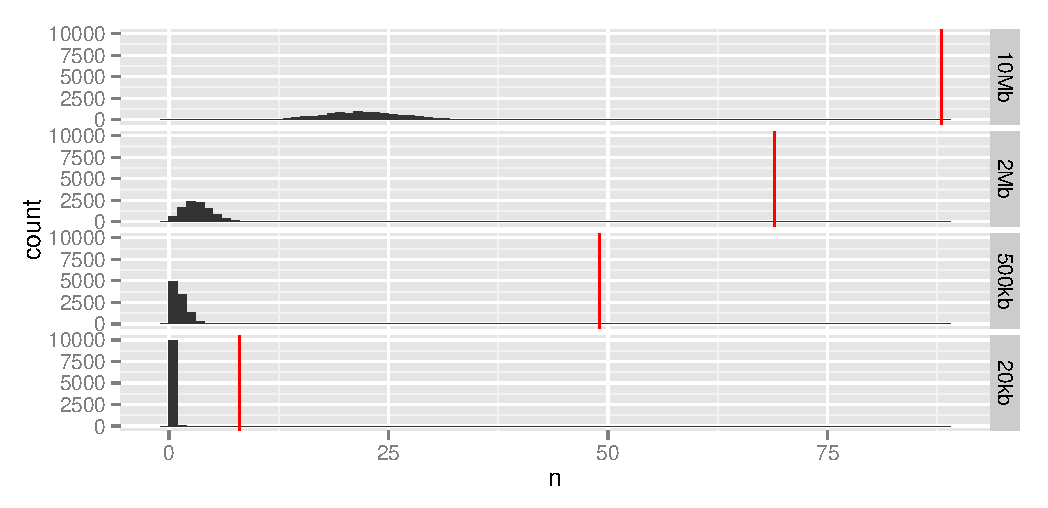
\includegraphics[width=5in]{chromosome_interactions}
	\caption{\textbf{Number of overlaps between chromosome interactions and epistatic interactions} Interacting chromosome regions may be a possible mechanism underlying epistatic interactions. The number of epistatic interactions within 20kb, 500kb, 2Mb and 10Mb of known chromosome interacting regions are shown by red vertical lines. The histograms represent the null distribution based on random sampling of 10000 datasets for each window size.}
	\label{fig:chromosomeinteractions}
\end{figure}
\clearpage

\begin{figure}
	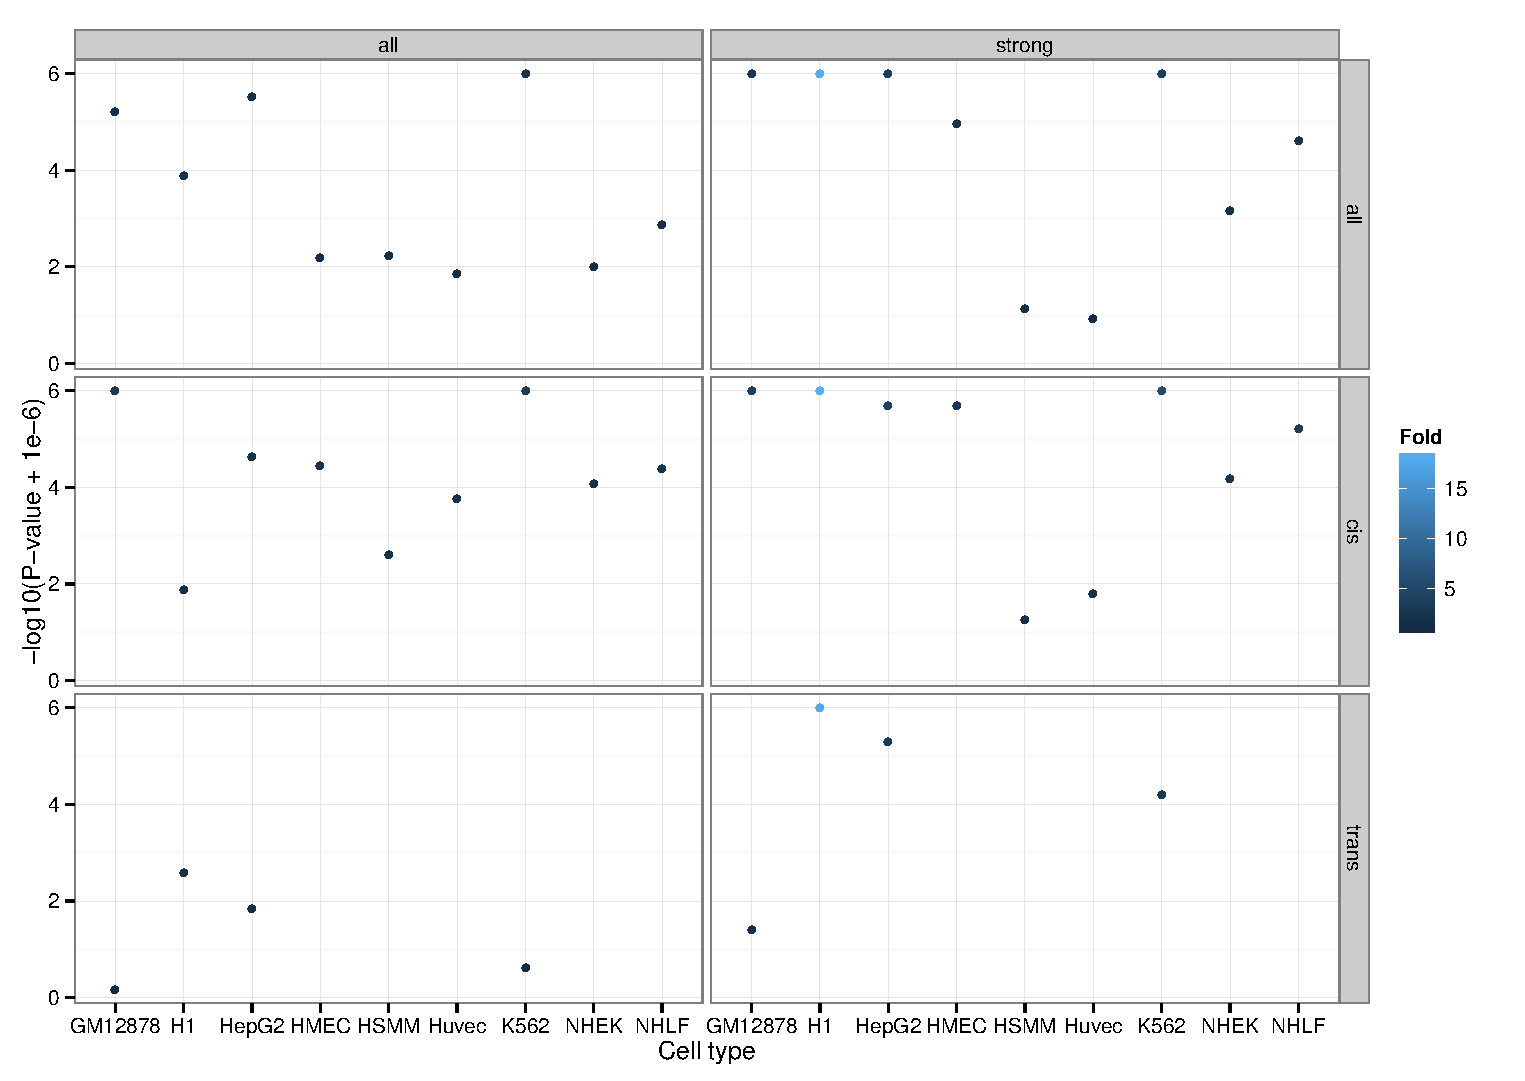
\includegraphics[width=5in]{enhancers}
	\caption{\textbf{There is enrichment for enhancer sequences for \emph{cis} and \emph{trans} SNPs}}
	\label{fig:enhancers}
\end{figure}
\clearpage

\end{document}